\subsection{Need for evaluation and basic definitions}

So far, we looked at the following supervised learning setting:
\begin{align*}
  \begin{array}{ccc}
    & \longrightarrow\\
    \text{descriptive features}& \quad
    \begin{array}{c}
      \text{\tiny Naive Bayes Classifier}\\
      \text{\tiny (Logistic) Regression}\\
      \text{\tiny Support Vector Machines}\\
      \text{\tiny Neural Networks}\\
      \text{\tiny ...}\\
    \end{array}\quad&\text{target feature}\\
    &\longrightarrow
  \end{array}
\end{align*}
\begin{itemize}
  \item We only distinguished between \textbf{training instances} and \textbf{unseen instances}
  \item An important introduced challenge is the occurrence of \textbf{over- and underfitting}
\end{itemize}

\begin{figure}[H]
  \centering
  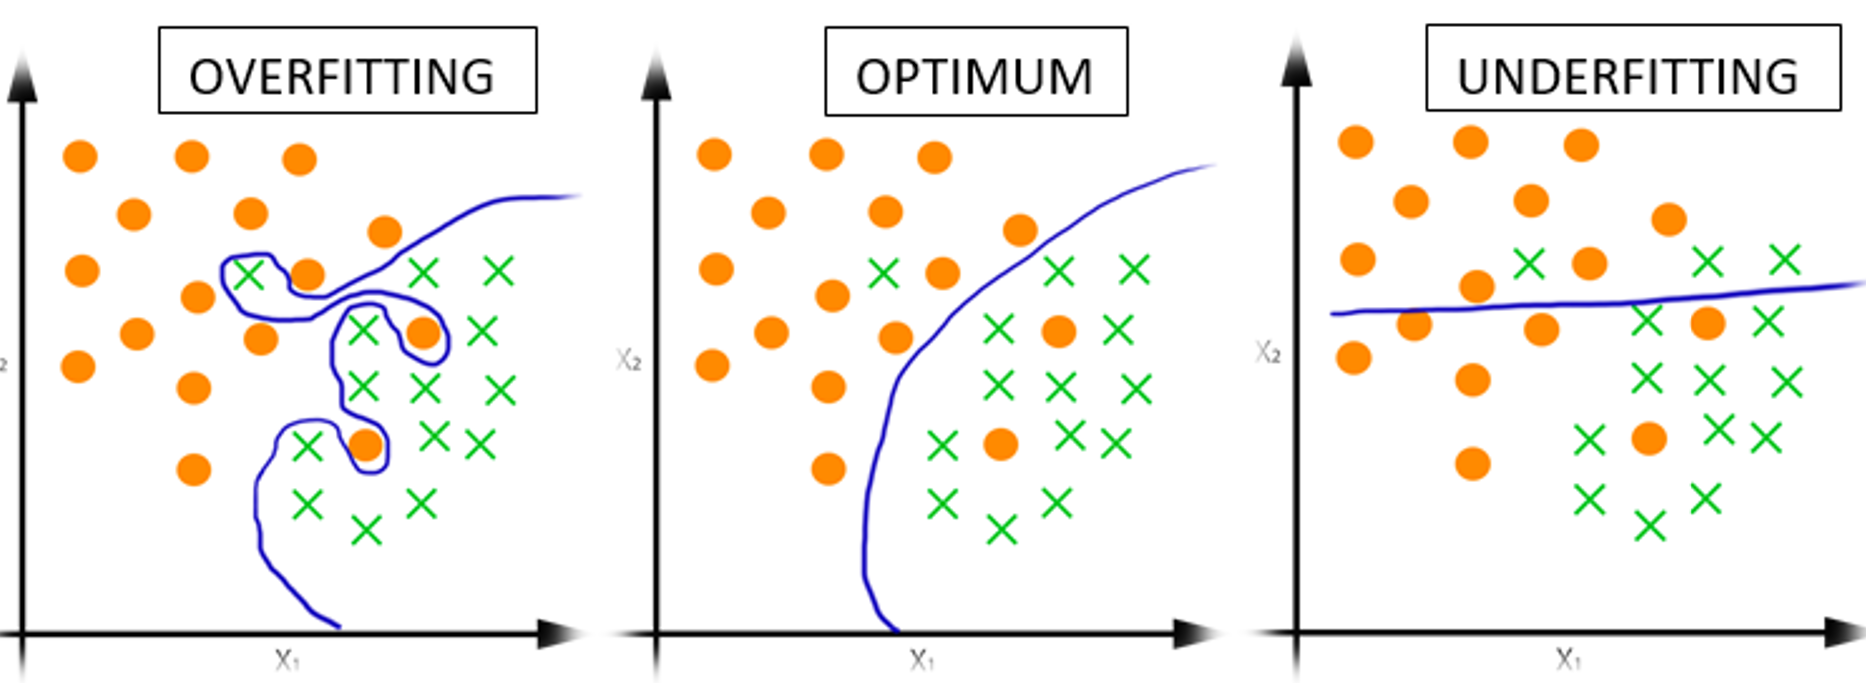
\includegraphics[width=0.45\textwidth]{assets/sl/basic__over_under_principle.png}
  \hspace*{0.05\textwidth}
  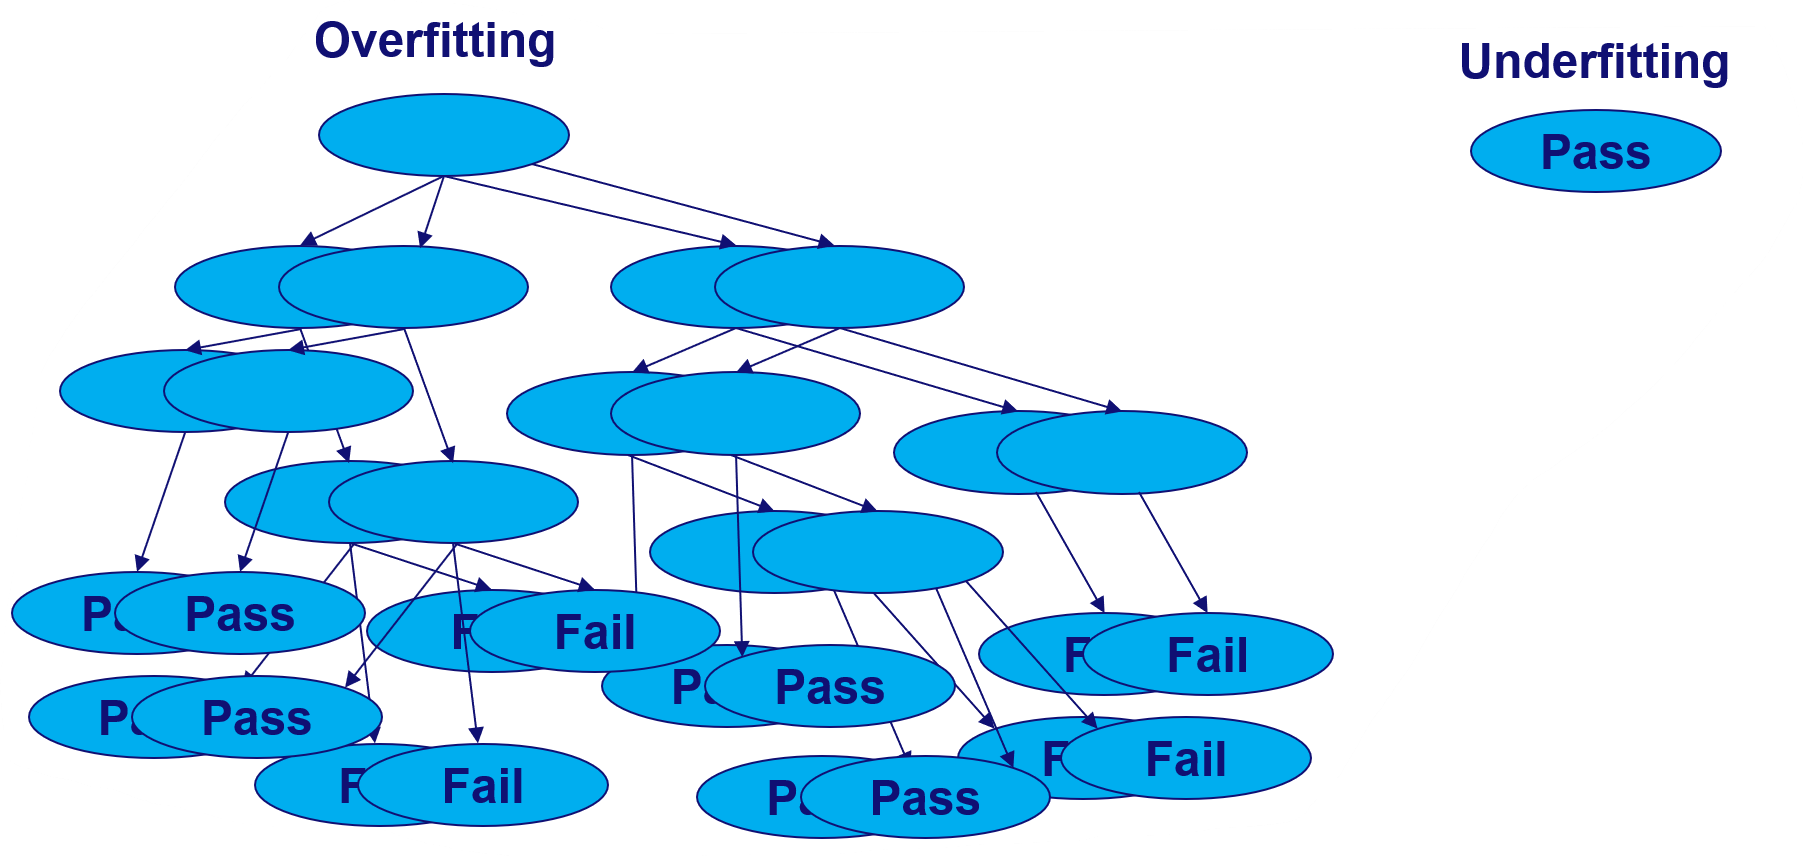
\includegraphics[width=0.45\textwidth]{assets/sl/basic__over_under_dt.png}

  \caption{Over- and underfitting}
  \label{fig:7_over_under_fitting}
\end{figure}

What we now want to introduce is a \textbf{hold-out test set}\sidenote{Test set}. Instead of using all of the collected labeled training data for actual training, we split it into a "true" training set and a validation set, which is then used for parameter selection, hyperparameter tuning, stopping criteria, etc.

\begin{figure}[H]
  \centering
  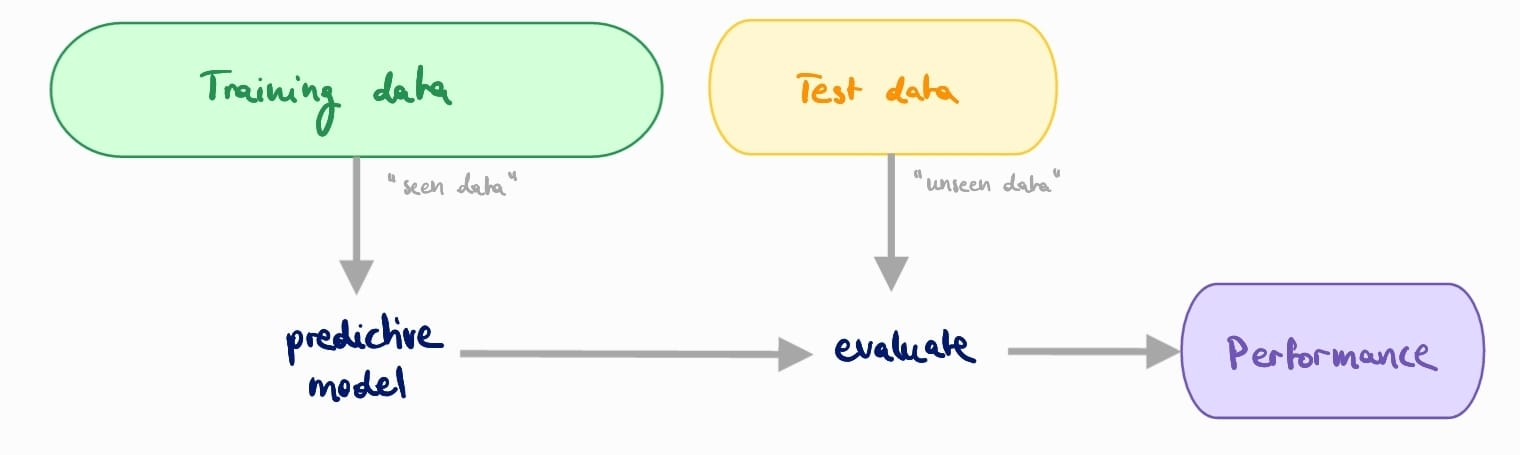
\includegraphics[width=0.9\textwidth]{assets/sl/basic__performance.jpg}
  \caption{Idea of test set and performance evaluation}
  \label{fig:7_test_set_principle}
\end{figure}

We're gonna look at an example of binary classification:
\begin{itemize}
  \item After training the network, we can evaluate its performance using the \textbf{confusion matrix}
  \item For that, take instances of the test set, apply them on the network, and compare the calculated result and the target
  \item This leads to the possible combination of:\sidenote{Confusion matrix}
  \begin{align*}
    TP: & \text{ True positive } \begin{array}{l}\text{\tiny result and target}\\\text{\tiny are both "positive"}\end{array}
      & FN: & \text{ False negative }  \begin{array}{l}\text{\tiny target is "positive", but}\\\text{\tiny the prediction "negative"}\end{array}\\
    FP: & \text{ False positive } \begin{array}{l}\text{\tiny target is "negative", but}\\\text{\tiny the prediction "positive"}\end{array} 
      & TN: & \text{ True negative } \begin{array}{l}\text{\tiny result and target}\\\text{\tiny are both "negative"}\end{array}
  \end{align*}
  \item For the confusion matrix, simply count the amount of $TP$, $FN$, $FP$, and $TN$ occurrences over all test set instances
  \item We can then have the misclassification accuracy calculated as 
  \begin{align*}
    acc = \frac{FP+FN}{TP+TN+FP+FN}
  \end{align*}
\end{itemize}

Next, we'll look at the \textbf{validation set}\sidenote{Validation set}. Instead of just having a test set, it is also possible to have a validation set that "pre-evaluates" the trained model. This again is for parameter optimization, model selection, or stopping criterion.
\begin{itemize}
  \item One may train hundreds of models using training data, and then select one model that performs well on the validation set, or
  \item One can stop iterating before the model starts to overfit the training data ("self-reflection")
\end{itemize}

\begin{figure}[H]
  \centering
  \begin{subfigure}{0.45\textwidth}
    \centering
    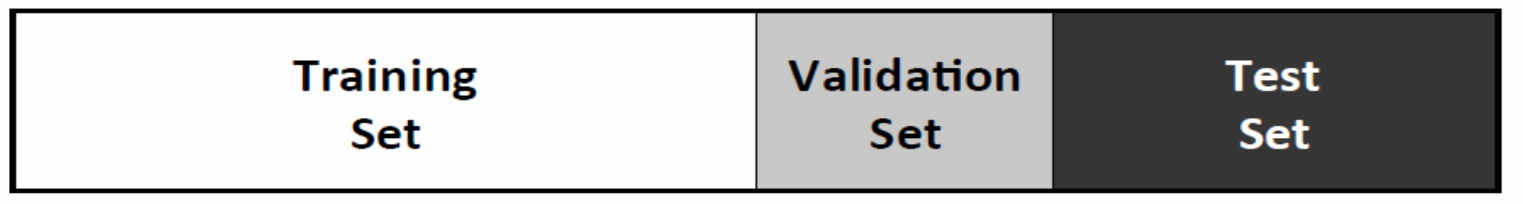
\includegraphics[width=\textwidth]{assets/sl/basic__data_split.png}
    \subcaption*{Typical splits are $50:20:30$ or $40:20:40$}
  \end{subfigure}
  \hspace*{0.05\textwidth}
  \begin{subfigure}{0.45\textwidth}
    \centering
    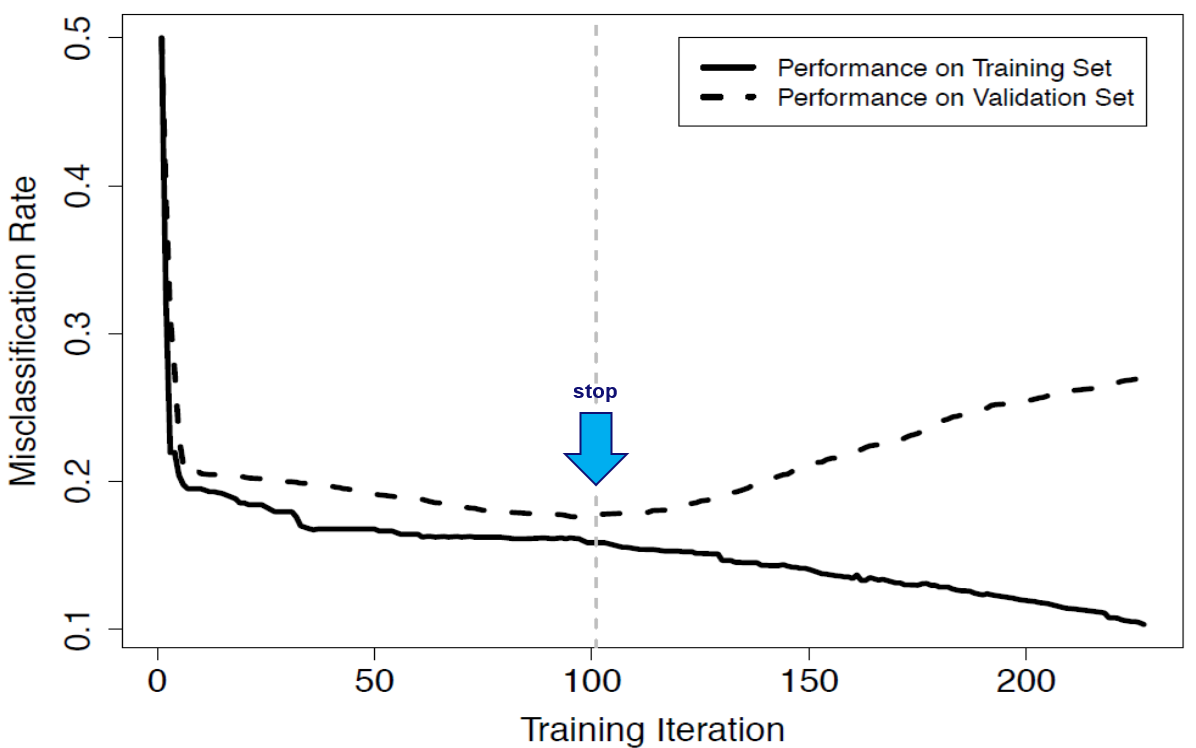
\includegraphics[width=\textwidth]{assets/sl/basic__validation_set_cutoff.png}
    \subcaption*{Validation set is used to avoid overfitting the test set}
  \end{subfigure}

  \caption{Idea of test set and performance evaluation}
  \label{fig:7_validation_set_split}
\end{figure}

From now on, we will abstract from the validation set and only consider training and test data.

